\documentclass{article}
\usepackage[utf8]{inputenc}

\title{\textbf{\textsc{Implementation of T Flip-Flop using 7474 IC}}}
\author{\textit{\textbf{Cheenepalli Chandana}}}
\usepackage{graphicx}
\begin{document}

\maketitle
\section{Abstract}
This manual shows Implementation of T flip-flop using 7474 IC
\section{Components}
% Please add the following required packages to your document preamble:
% \usepackage{graphicx}
\begin{table}[ht]
\resizebox{\columnwidth}{!}{%
\begin{tabular}{|l|l|l|}
\hline
\textbf{Component} & \textbf{Value} & \textbf{Quantity} \\ \hline
Bread board & - & 1 \\ \hline
Arduino & Uno & 1 \\ \hline
LED & - & 2 \\ \hline
IC & 7474 & 1 \\ \hline
Jumper Wires & - & 20 \\ \hline
\end{tabular}%
}
\caption{}
\label{Tabel-1}
\end{table}
\section{Procedure}
1.consider four digital pins 13,7,2,4,7 as input and 2,4 as ouputs .
\\
2.here D13 acts as clock signal 
\\
3.connect 7474(1,4:VCC) to deactivate them otherwise they will interrupt in output
\\
4.connect 7474(7:GND &14:VCC)
\\
5.connect 7474(2:7,5:4) and take slider switch as toggle input connect it to D2.
\\
6.D=T&&!Q || !T&&Q.
\\
7.Connect another LED +  to the 5 (Q) pin of the IC 7474 and GND the other terminal.
\\
8.Change the D2 pin in the Arduino  from VCC to GND and observe the outputs.
\\

\section{Code}
Execute the following code using the below provided link
\\
\begin{table}[ht]
\resizebox{\columnwidth}{!}{%
\begin{tabular}{|l|}
\hline
https://github.com/chandana531/cchandana_fwc/blob/main/assignment1_assembly/codes/ide.ino
\end{tabular}%
}
\end{table}
% Please add the following required packages to your document preamble:
% \usepackage{graphicx}
\section{Conversion table}
\begin{table}[ht]
\centering
\resizebox{\textwidth}{!}{%
\begin{tabular}{|l|lll|ll|}
\hline
\textbf{Input} & \multicolumn{3}{l|}{\textbf{Intermediate Inputs}} & \multicolumn{2}{l|}{\textbf{Outputs}} \\ \hline
T & \multicolumn{1}{l|}{Qn} & \multicolumn{1}{l|}{!Qn} & T=D xor Qn & \multicolumn{1}{l|}{Qn} & !Qn \\ \hline
0 & \multicolumn{1}{l|}{0} & \multicolumn{1}{l|}{1} & 0 & \multicolumn{1}{l|}{0} & 1 \\ \hline
0 & \multicolumn{1}{l|}{1} & \multicolumn{1}{l|}{0} & 1 & \multicolumn{1}{l|}{1} & 0 \\ \hline
1 & \multicolumn{1}{l|}{0} & \multicolumn{1}{l|}{1} & 1 & \multicolumn{1}{l|}{1} & 0 \\ \hline
1 & \multicolumn{1}{l|}{1} & \multicolumn{1}{l|}{0} & 0 & \multicolumn{1}{l|}{0} & 1 \\ \hline
\end{tabular}%
}
\caption{}
\label{conversion table}
\end{table}


\begin{figure}
	\centering																	   		
	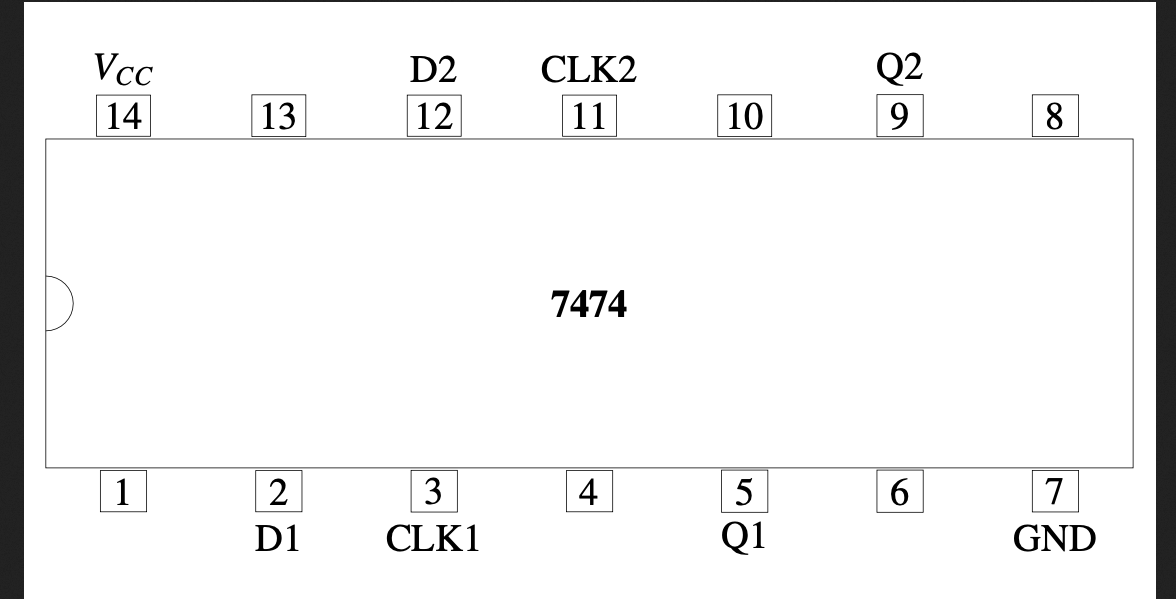
\includegraphics[width=3in]{ic.png}
	\caption{7474}
	\label{fig:circuit}	
\end{figure}
\begin{figure}
	\centering
	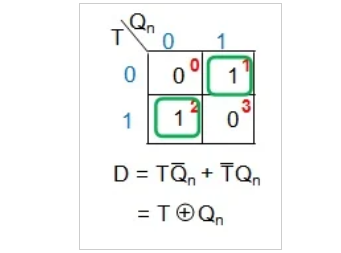
\includegraphics[width=3in]{kmap.png}
	\caption{kmap}
	\label{fig:circuit}
\end{figure}



\begin{figure}
\centering
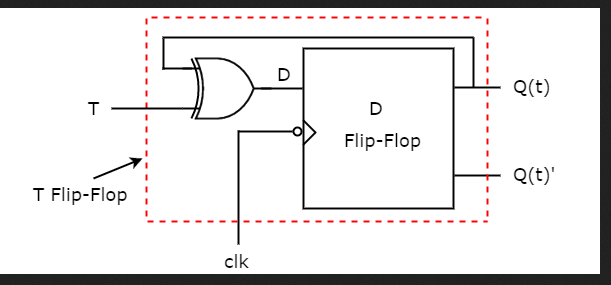
\includegraphics[width=3in]{T_flipflop.png}
\caption{Circuit Diagram}

\end{figure}



\end{document}